\chapter{Process Configuration}
\label{sec:config}
In this section I show each step of process configuration. At the same time I describe my implementation of the 
\emph{reducer tree} and \emph{tuner network} data structures.

\subsection{Defining the Reducer Tree}
A \emph{reducer tree} can be constructed expediently using existing \emph{geometry} and \emph{material node} types.
\emph{Reducer trees} are not restricted to use only existing node types.
New node types can be added by extending the \verb|ReducerNode| class (see Figure~\ref{fig:node}).
In particular, implementing a new \emph{geometry node} type requires providing the function \verb|getOutputIndex|.
This function takes, as input, a 3D position and returns the \verb|id| of its child (Geometry or Material)
that contains this 3D point.
This function also computes a local coordinate for this child node.
Performing computations in local coordinates allows us to abstract away the geometry of a given object.
Implementing a new \verb|MaterialNode| type requires specifying the \verb|getMaterial| function
which takes a 3D point and returns the material at this point in the local geometry coordinate system.
Both types of nodes have an \verb|evaluate| function which is responsible for updating their internal states.
This function is used by the \emph{tuner network} to modify the internal state of the nodes.
As an example, we show a \emph{reducer tree} for performing texture mapping (see Figure~\ref{fig:red1}).
We also provide the corresponding pseudo-code (see Algorithm~\ref{alg:ReducerTree}).

% Nodes also posses a \textit{getSearchSpace} virtual function which is used by the Tuner to retrieve the all tunable variables in the nodes subtree. In order to allow efficient computation of surface properties we provide each node with a \textit{getMesh} method which can return a triangular surface mesh of a subtree. Certain simulators require surface normal information to produce results and this can be efficiently computed from the provided surface mesh.

\begin{figure}[h]
\centering
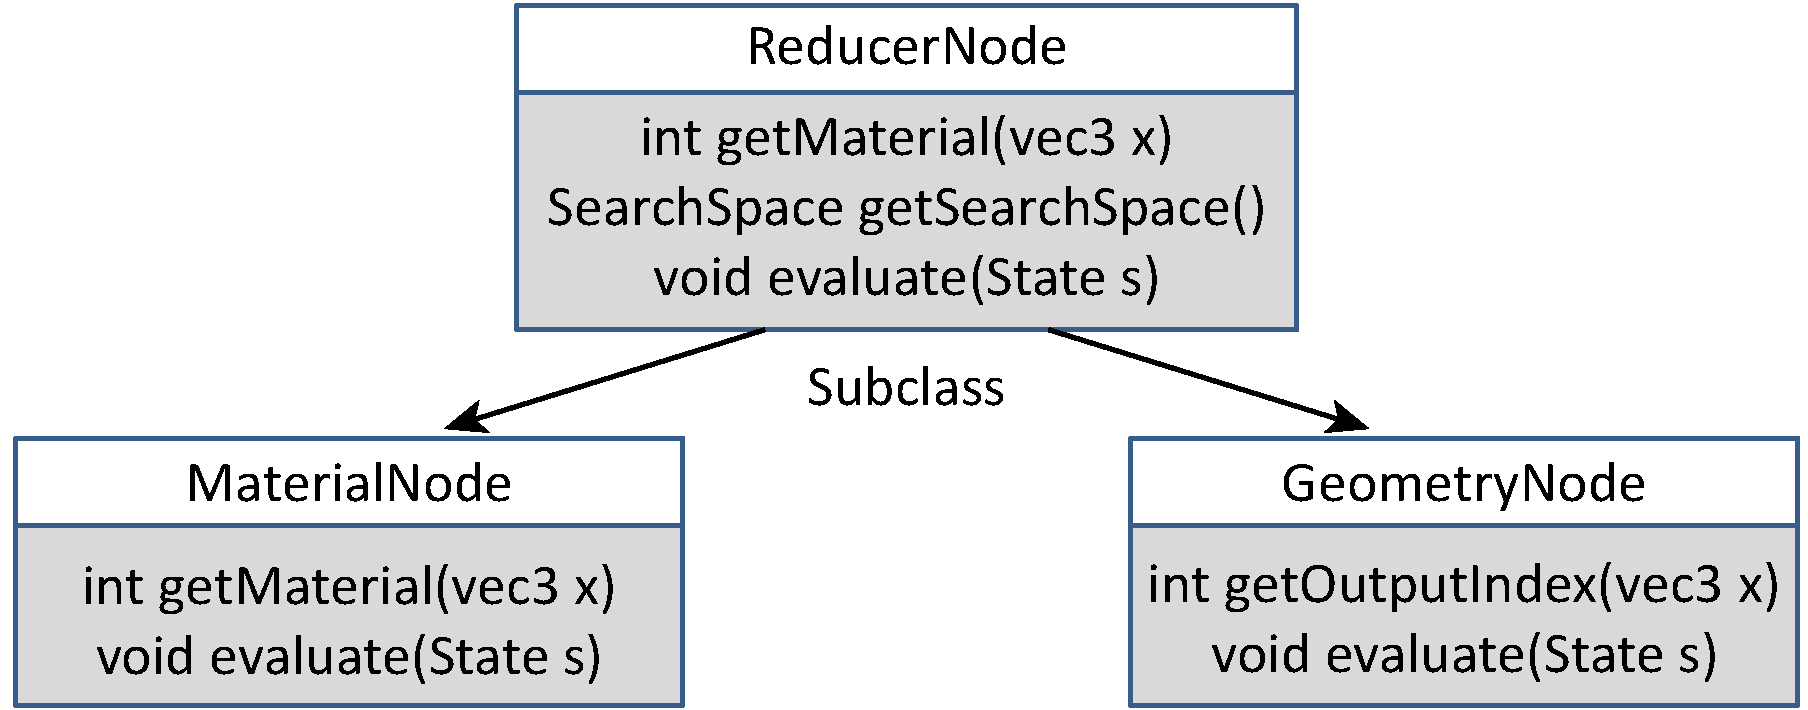
\includegraphics[width=\linewidth]{figure/node.pdf}
\caption{Abstract interface for Node and its two subclasses.}
\label{fig:node}
\end{figure}

\begin{algorithm}
\caption{Constructing a \emph{reducer tree} for texturing}
\label{alg:ReducerTree}
\begin{lstlisting}[mathescape=true]
1. Create a root node $\mathbf{R}$ from inputMesh 
2. Subdivide $\mathbf{R}$ into outer layer $\mathbf{O}$ and inner volume $\mathbf{V}$ (Stratum Node) 
3. Subdivide $\mathbf{O}$ into set of columns $\mathbf{C}$ 
    (Column Node) 
4. For each column $\mathbf{c}$ in $\mathbf{C}$ 
5.   Subdivide $\mathbf{c}$ into two layers 
      (Layer Node) 
6. End 
\end{lstlisting}
\end{algorithm}

\subsection{Defining a \emph{Tuner}}
Recall that a \emph{tuner} consists of four components: a simulation, an error metric, an optimizer and a goal (\autoref{fig:tuner0}). Certain combinations of goal, metric and simulator are not compatible (i.e., a deformation simulator is not compatible with an error metric that compares images). Our API checks and prevents such incompatible combinations of components.  The optimization algorithm can request the error value for a given state using a callback function \verb|getError()| which is defined by the \emph{tuner}. Additional callback functions can be defined by the developer depending on the needs of the algorithm. For example, the branch and bound algorithm requires a custom  function to compute error bounds for a given state.
%Once a suitable set of components has been chosen they can be easily combined (Algorithm~\ref{alg:Tuner}).

%\begin{algorithm}
%\caption{Configuring a Tuner}
%\label{alg:Tuner}
%\begin{verbatim}
%1. Set Tuner's optimizer to ColorOptimizer
%2. Set Tuner's error metric to L1 distance
%3. Set Tuner's simulator to ColorSimulator
%\end{verbatim}
%\end{algorithm}

\subsection{Binding \emph{Tuners}}

\emph{Tuners} are assigned to nodes in the \emph{reducer tree} using the \verb|setNode| function. Once assigned, a \emph{tuner} can optimize the parameters of its associated subtree. \emph{Reducer nodes} provide a \verb|getSearchSpace| function which returns all free variables in the node subtree. In order to make \emph{tuners} as flexible as possible we provide a \verb|Parameter| class. Parameters can be either discrete or continuous, they can have associated bounds, and they can be marked as free or fixed.

\subsection{Establishing the \emph{Tuner Network}}

The \emph{tuner network} is an undirected graph that describes connections between \emph{tuners}. \emph{Tuner nodes} store a list of their neighbors. Only neighboring \emph{tuners} are allowed to exchange information. In our current implementation, this is accomplished using a shared memory array. As an example, we show how to construct and initialize a \emph{tuner network} for a simple optimization scheme -- a Simulated Annealing algorithm~\cite{Van:1987} (see Algorithm~\ref{alg:TunerNetwork}). The \emph{tuner network} also requires a schedule that specifies in what order individual \emph{tuners} should be executed. This schedule is specified by the developer. Once the \emph{tuner network} is constructed, the process configuration phase is complete. We obtain a compiled executable that computes desired material assignment from an input specification.
\begin{algorithm}
\caption{Connecting and executing the \emph{tuner network}}
\label{alg:TunerNetwork}
\begin{lstlisting}[mathescape=true]
1.  for each Tuner $\mathbf{T}_i$ attached to a plane
2.    for each Tuner $\mathbf{T}_j$ adjacent to $\mathbf{T}_i$
3.      add $\mathbf{T}_j$ to $\mathbf{T}_i$'s list of neighbors
4.    end
5.  end
6.  iterate N times
7.  for each Tuner $\mathbf{T}_i$
8.    set temperature for $\mathbf{T}_i$'s optimizer
9.    run $\mathbf{T}_i$
10. end
\end{lstlisting}
\end{algorithm} 
\section{Process Use}
\label{sec:use}
The compiled program, which executes the \emph{tuner network}, takes five types of arguments: the input geometry, the goal, the simulation configuration, a set of materials and the target 3D printer specification. 
After the \emph{tuner network} is executed, the parameters of the \emph{reducer nodes} in the \emph{reducer tree} are set. It is then straightforward to compute the material assignment at arbitrary resolution. Since, a typical multi-material 3D printer requires a volumetric model with per voxel material assignment, we can simply iterate over all voxels in the volume. We obtain the material assignment by evaluating (\verb|getMaterial|) of the \emph{reducer tree} root at the center of each voxel location. This representation can be easily converted to a printer specific format for output. For the Objet500 Connex printer used in this paper we extract material isosurfaces which are submitted to the printer as STL files. 